\begin{table}[h!]
\section{Funktionsgraphen}
\begin{center}
	\begin{tabularx}{550pt}{c X c X c X}
%	e-Funktion & Logarithmusfunktion & $\frac{1}{x}- Funktion$\\
	
%	\raisebox{-.7\totalheight}{\includegraphics[width = 3.5cm]{../bilder/2_Efunktion.png}} & \raisebox{-.7\totalheight}{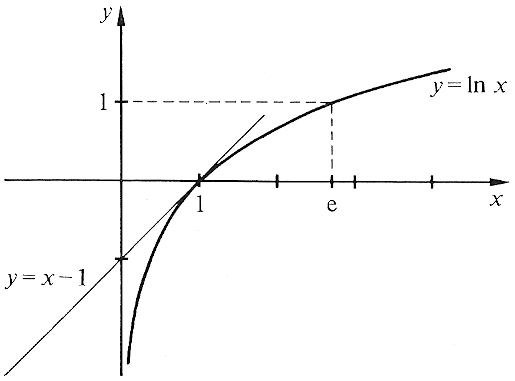
\includegraphics[width =  5cm]{../bilder/2_lnFunktion.png}}&
%	\raisebox{-.7\totalheight}{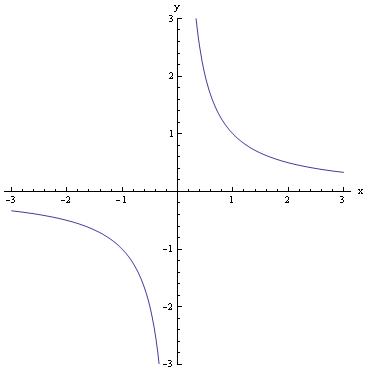
\includegraphics[width = 3.5cm]{../bilder/2_1toxFunktion.png}} \\


	Trigo-Funktionen & Arcus-Funktion &  Hyperbel-Funktionen\\
	
	\raisebox{-.7\totalheight}{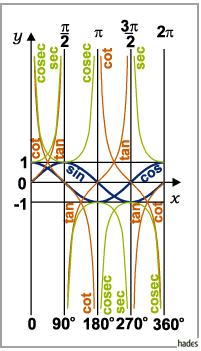
\includegraphics[width= 4.8cm]{bilder/2_trigoFunktionen.png}} & \raisebox{-.7\totalheight}{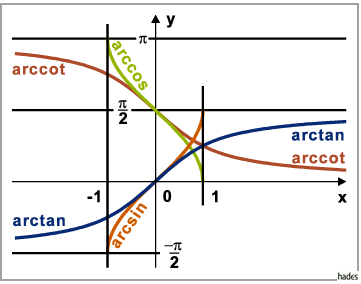
\includegraphics[width =  7cm]{bilder/2_arcusFunktionen.png}}&
	\raisebox{-.7\totalheight}{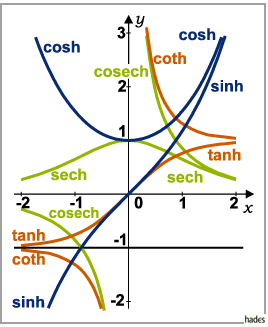
\includegraphics[width = 6.5cm]{bilder/2_hyperbel.png}} \\
\end{tabularx}
\end{center}
\end{table}
